\documentclass[12pt, twoside]{book}
%\documentclass[12pt, oneside]{book}  % jednostranna tlac

%spravne nastavenie okrajov
\usepackage[a4paper,top=2.5cm,bottom=2.5cm,left=3.5cm,right=2cm]{geometry}
%zapnutie fontov pre UTF8 kodovanie
\usepackage[utf8]{inputenc}
\usepackage[T1]{fontenc}
\usepackage{amsmath}

%zapnutie slovenskeho delenia slov
%a automatickych nadpisov ako Obsah, Obrázok a pod. v slovencine
\usepackage[slovak]{babel} % vypnite pre prace v anglictine!

%nastavenie riadkovania podla smernice
\linespread{1.25} % hodnota 1.25 by mala zodpovedat 1.5 riadkovaniu

% balicek na vkladanie zdrojoveho kodu
\usepackage{listings}
% ukazky kodu su cislovane ako Listing 1,2,...
% tu je Listing zmenene na Algoritmus 1,2,...
\renewcommand{\lstlistingname}{Algoritmus}
% nastavenia balicka listings
% mozete pridat aj language=...
% na nastavenie najcastejsie pouzivaneho prog. jazyka
% takisto sa da zapnut cislovanie riadkov
\lstset{frame=lines}

% balicek na vkladanie obrazkov
\usepackage{graphicx}
% balicek na vkladanie celych pdf dokumentov, tu zadanie
\usepackage{pdfpages}
% balicek na spravne formatovanie URL
\usepackage{url}
% balicek na hyperlinky v ramci dokumentu
% zrusime farebne ramiky okolo liniek aby pdf
% vyzeralo rovnako ako tlacena verzia
\usepackage[hidelinks,breaklinks]{hyperref}



% -------------------
% --- Definicia zakladnych pojmov
% --- Vyplnte podla vasho zadania, rok ma byt rok odovzdania
% -------------------
\def\mfrok{2024}
\def\mfnazov{Trénovanie autonómneho vozidla v hre Trackmania pomocou strojového učenia}
\def\mftyp{Bakalárska práca}
\def\mfautor{Timotej Melkovič}
\def\mfskolitel{Mgr. Iveta Bečková}

%ak mate konzultanta, odkomentujte aj jeho meno na titulnom liste
\def\mfkonzultant{tit. Meno Priezvisko, tit. }  

\def\mfmiesto{Bratislava, \mfrok}

% študenti BIN a DAV odkomentujú príslušnú dvojicu riadkov
\def\mfodbor{ Informatika }
\def\program{ Aplikovaná informatika }
% pre BIN:
%\def\mfodbor{ Informatika a Biológia }
%\def\program{ Bioinformatika }
% pre DAV:
%\def\mfodbor{ Informatika a Matematika } 
%\def\program{ Dátová veda }

% Ak je školiteľ z FMFI, uvádzate katedru školiteľa, zrejme by mala byť aj na zadaní z AIS2
% Ak máte externého školiteľa, uvádzajte Katedru informatiky 
\def\mfpracovisko{ Katedra informatiky }


\begin{document} 


\frontmatter
\pagestyle{empty}

% -------------------
% --- Obalka ------
% -------------------

\begin{center}
\sc\large
Univerzita Komenského v Bratislave\\
Fakulta matematiky, fyziky a informatiky

\vfill

{\LARGE\mfnazov}\\
\mftyp
\end{center}

\vfill

{\sc\large 
\noindent \mfrok\\
\mfautor
}

\cleardoublepage
% --- koniec obalky ----

% -------------------
% --- Titulný list
% -------------------


\noindent

\begin{center}
\sc  
\large
Univerzita Komenského v Bratislave\\
Fakulta matematiky, fyziky a informatiky

\vfill

{\LARGE\mfnazov}\\
\mftyp
\end{center}

\vfill

\noindent
\begin{tabular}{ll}
Študijný program: & \program \\
Študijný odbor: & \mfodbor \\
Školiace pracovisko: & \mfpracovisko \\
Školiteľ: & \mfskolitel \\
% Konzultant: & \mfkonzultant \\
\end{tabular}

\vfill


\noindent \mfmiesto\\
\mfautor

\cleardoublepage
% --- Koniec titulnej strany


% -------------------
% --- Zadanie z AIS
% -------------------
% v tlačenej verzii s podpismi zainteresovaných osôb.
% v elektronickej verzii sa zverejňuje zadanie bez podpisov
% v pracach v angličtine anglické aj slovenské zadanie

\newpage 
\setcounter{page}{1}
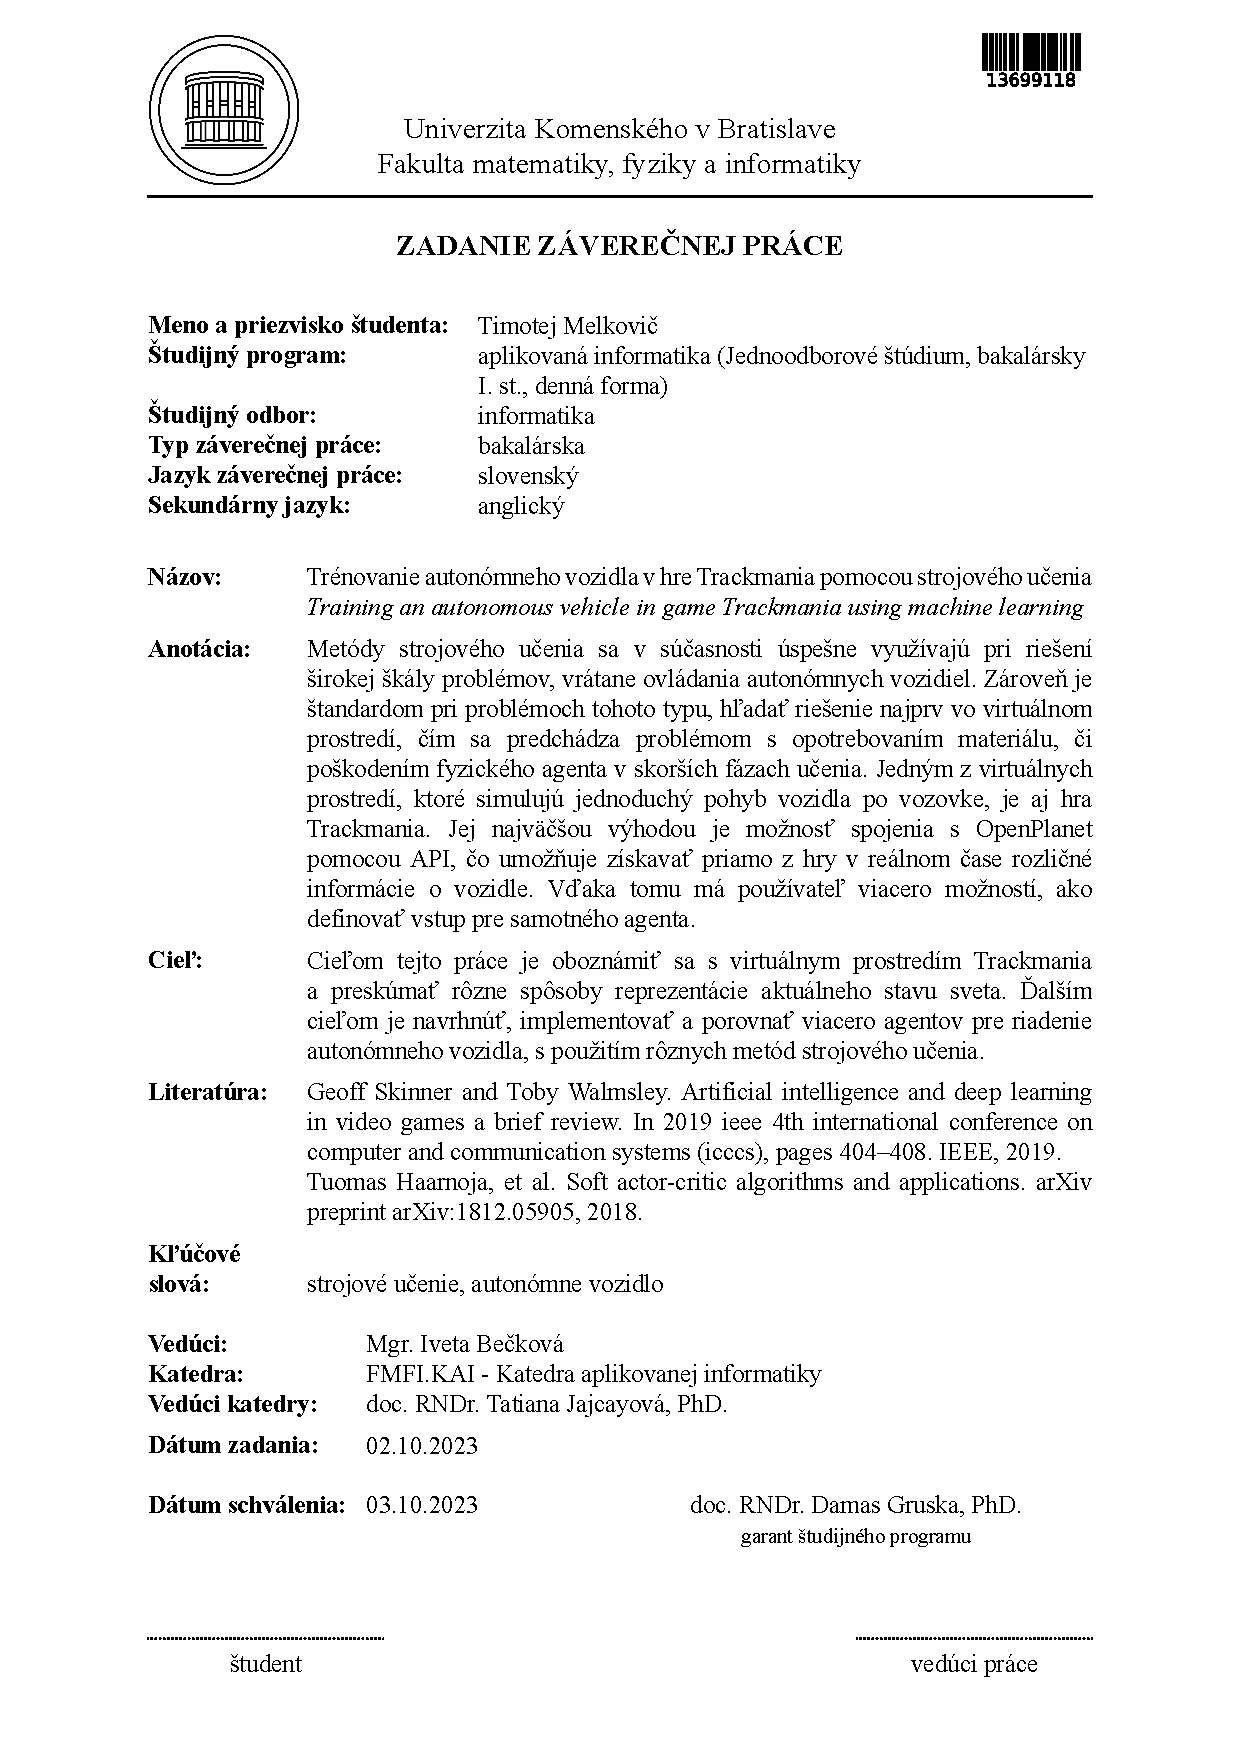
\includepdf{images/zadanie.pdf}

% --- Koniec zadania
\newpage 
\noindent 
\pagestyle{empty}
~


% -------------------
%   Poďakovanie - nepovinné
% -------------------
\newpage 
\pagestyle{plain}
~

\vfill
{\bf Poďakovanie:} Týmto spôsobom by som sa chcel srdečne poďakovať svojej školiteľke, Mgr. Ivete Bečkovej, za odovzdané vedomosti a rady, ako aj za jej veľkú trpezlivosť počas celého obdobia riešenia bakalárskej práce. Jej odborné vedenie a zodpovedný prístup boli neoceniteľné a výrazne prispeli k úspešnému dokončeniu tejto práce.

% --- Koniec poďakovania

% -------------------
%   Abstrakt - Slovensky
% -------------------
\newpage 
\section*{Abstrakt}

Metódy strojového učenia sa v súčasnosti úspešne využívajú pri riešení širokej škály problémov, vrátane ovládania autonómnych vozidiel. Táto práca sa zameriava na implementáciu autonómneho agenta pre hru Trackmania, ktorá poskytuje virtuálne prostredie na trénovanie a testovanie pokročilých algoritmov umelej inteligencie. Cieľom bolo vytvoriť agenta schopného dokončiť pretekársku trať bez ľudského zásahu, pričom sa využívajú metódy učenia posilňovaním a raycastingu na simuláciu senzorov. Výsledky ukazujú, že agent je schopný úspešne dokončiť trate s vysokou konzistenciou výsledkov, aj keď nedosahuje úroveň skúsených hráčov. Práca tiež navrhuje možné smery pre ďalší výskum a zlepšovanie autonómnych agentov v hre Trackmania.
\\
\\
\textbf{Kľúčové slová:} strojové učenie, autonómne vozidlo, Trackmania, učenie posilňovaním

% --- Koniec Abstrakt - Slovensky


% -------------------
% --- Abstrakt - Anglicky 
% -------------------
\newpage 
\section*{Abstract}

Machine learning methods are currently successfully used to solve a wide range of problems, including controlling autonomous vehicles. This thesis focuses on the implementation of an autonomous agent for the game Trackmania, which provides a virtual environment for training and testing advanced artificial intelligence algorithms. The goal was to create an agent capable of completing a racing track without human intervention, using reinforcement learning and raycasting methods to simulate sensory perceptions. The results show that the agent can successfully complete tracks with high consistency, although it does not reach the level of experienced players. The work also suggests possible directions for further research and improvement of autonomous agents in game Trackmania.
\\
\\
\textbf{Keywords:} machine learning, autonomous vehicle, Trackmania, reinforcement learning, raycasting


% --- Koniec Abstrakt - Anglicky

% -------------------
% --- Predhovor - v informatike sa zvacsa nepouziva
% -------------------
%\newpage 
%
%\chapter*{Predhovor}
%
%Predhovor je všeobecná informácia o práci, obsahuje hlavnú charakteristiku práce 
%a okolnosti jej vzniku. Autor zdôvodní výber témy, stručne informuje o cieľoch 
%a význame práce, spomenie domáci a zahraničný kontext, komu je práca určená, 
%použité metódy, stav poznania; autor stručne charakterizuje svoj prístup a svoje 
%hľadisko. 
%
% --- Koniec Predhovor


% -------------------
% --- Obsah
% -------------------

\newpage 

\tableofcontents

% ---  Koniec Obsahu

% -------------------
% --- Zoznamy tabuliek, obrázkov - nepovinne
% -------------------

\newpage 

\listoffigures
\listoftables

% ---  Koniec Zoznamov

\mainmatter
\pagestyle{headings}


\input uvod.tex 

\input teoria.tex

\input navrh.tex

\input praktika.tex

\input vyhodnotenie.tex

\input zaver.tex

% -------------------
% --- Bibliografia
% -------------------


\newpage	

\backmatter

\thispagestyle{empty}
\clearpage

\bibliographystyle{plain}
\bibliography{literatura} 

%Prípadne môžete napísať literatúru priamo tu
%\begin{thebibliography}{5}
 
%\bibitem{br1} MOLINA H. G. - ULLMAN J. D. - WIDOM J., 2002, Database Systems, Upper Saddle River : Prentice-Hall, 2002, 1119 s., Pearson International edition, 0-13-098043-9

%\bibitem{br2} MOLINA H. G. - ULLMAN J. D. - WIDOM J., 2000 , Databasse System implementation, New Jersey : Prentice-Hall, 2000, 653s., ???

%\bibitem{br3} ULLMAN J. D. - WIDOM J., 1997, A First Course in Database Systems, New Jersey : Prentice-Hall, 1997, 470s., 

%\bibitem{br4} PREFUSE, 2007, The Prefuse visualization toolkit,  [online] Dostupné na internete: <http://prefuse.org/>

%\bibitem{br5} PREFUSE Forum, Sourceforge - Prefuse Forum,  [online] Dostupné na internete: <http://sourceforge.net/projects/prefuse/>

%\end{thebibliography}

%---koniec Referencii

% -------------------
%--- Prilohy---
% -------------------

%Nepovinná časť prílohy obsahuje materiály, ktoré neboli zaradené priamo  do textu. Každá príloha sa začína na novej strane.
%Zoznam príloh je súčasťou obsahu.
%
\input appendixA.tex

%\input appendixB.tex

\end{document}






